\documentclass[a4paper, norsk, 12pt]{article}

% General packages
\usepackage{parskip}      % Vertical space on new paragraph instead of indent
\usepackage{hyperref}   % For including links
\usepackage{url}          % Allows adding url's
\usepackage[top=4cm, bottom=4cm]{geometry}     % Easier management of page dimensions
\usepackage{chngcntr}     % Customizable counters
\usepackage{enumitem}     % Can use [noitemsep] on lists to reduce spacing
\usepackage{fancyhdr}
\pagestyle{fancy}
\usepackage{afterpage} 	% Various tweaks for page breaks and stuff
\usepackage{amsmath, amsthm}
\usepackage{babel}
\theoremstyle{remark}
\newtheorem{rem}{Remark}

% BEGIN Floats
\usepackage[bf, hang, small]{caption}	% Nicer captions for floats.
\usepackage{float}        % Allows advanced placement options for floats
\usepackage{mwe}    % loads »blindtext« and »graphicx«
\usepackage{subfig}		% Sub-figures. Crashes with captions package
% END Floats

% BEGIN Tables
\usepackage{booktabs}		% More professional looking tables
\usepackage{tabularx}		% Allows width adjustment etc. for tables
\usepackage{multirow}		% Allows table cells to span rows or columns
% END Tables

% Font specific packages
\usepackage{fontspec}
\usepackage{textcomp}
\usepackage{titlesec}
\usepackage{titling}
\usepackage{inconsolata}
\usepackage[default]{droidserif}

% Specifying fonts
\setsansfont{Open Sans}
\setmainfont[Scale=0.80]{Droid Serif}
\fontspec{Inconsolata}
\setmonofont[Scale=0.80]{Inconsolata}
\newfontfamily\headingfont[]{Open Sans}
\newfontfamily\headingfont[]{Open Sans}
\titleformat*{\section}{\Large\headingfont}
\titleformat*{\subsection}{\large\headingfont}
\titleformat*{\subsubsection}{\normalsize\headingfont}
\renewcommand{\maketitlehooka}{\headingfont}

% Title spacing
%\titlespacing{command}{left spacing}{before spacing}{after spacing}[right]
\titlespacing\section{0pt}{14pt}{0pt}
\titlespacing\subsection{0pt}{12pt}{0pt}
\titlespacing\subsubsection{0pt}{10pt}{0pt}

\usepackage{cite}



\title{TMM4220 Innovasjon \\ 
\vspace{6pt}\large Parkeringssystem for Oslo kommune \\ \vspace{50pt} 
 }

\author{Einar Baumann \\Elise Landsem\\D\v{z}enan Dumpor\\Magnus Rodahl\\Sigbjørn Aukland}   
\date{\today}

\begin{document}

\maketitle
\thispagestyle{empty}
\vspace{50pt}
\begin{abstract}
Sammendraget ...
\end{abstract}
\pagebreak

\tableofcontents
\pagebreak

\section*{Forord}
Problemstilling, formål, faget og sånt
\pagebreak



\section{Innledning}
\label{sec:innledning}
\cite{vekstbedriften}
% section innledning (end)




\section{Teori}
\label{sec:teori}

% section teori (end)





\section{Teknologiundersøkelse}
\label{sec:teknologi}

\subsection{Kriterier for idéelt system}
\label{sub:ideelt_system}
Gruppen ser for seg at en egenutviklet løsning må bestå av minimum følgende komponenter:

\begin{itemize}
	\item Sensorer med støtte for lesing RFID e.l. som graves ned i bakken. Detekterer biler som står over, og leser potensielt en form for ID-brikke.
	\item Enten “basestasjoner” som kommuniserer trådløst med sensorenhetene, eller omfattende kabelnettverk som knytter de sammen.
	\item Sentral database som lagrer informasjon om parkeringsplassene.
 	\item App e.l. for brukerne som lar de finne ledige parkeringsplasser og betale for parkering.
	\item App e.l. for paringsvakter som hjelper de til å finne frem til parkeringsavvik og registrere de.
	\item Administreringssystem for ymse ting.
\end{itemize}

\subsubsection{Sensorer}
\label{ssub:sensorer}
En mulig løsning for sensor er en kombinasjon av magnetometer og RFID-leser. Magnetometeret registrerer om det står en bil over, uavhengig om bilen har en ID-brikke eller ikke. RFID-leseren leser av ID-brikken dersom bilen har en.

Både magnetometer og RFID-lesere er moden teknologi som allerede er i bruk i parkeringssensorer i ekseisterende systemer. 
% subsubsection sensorer (end)

\subsubsection{App for brukere}
\label{ssub:app_for_brukere}
Bør oppfylle følgende kriterer:
\begin{itemize}
	\item Betaling gjennom app (start/stopp eller forhådsbestemt tidsrom).
	\item Finne ledige parkeringsplasser.
	\item Veldig brukervennlig.
\end{itemize}
% subsubsection app_for_brukere (end)

\subsubsection{App for kontrollører}
\label{ssub:kontrollor_app}
Samtaler med bymiljøetaten har avdekt at problemet med det eksisterende systemet er at det er oppdelt: vaktene må manuelt sjekke flere forskjellige registre for betalt parkering (kontant med lapp, app, sms...), betalt piggdekkavgift, etc.

Et nytt system bør gi mulighet for å sjekke samtlige ting samtidig. Eksempelvis kan man scanne nummerskiltet, og få opp OK/IKKE OK for hvert punkt. Dette innebærer at systemet for parkeringsbetalingen bør kunne knyttes sammen med noen eksisterende systemer.

Appen bør også kunne lede kontrollørene til parkeringsplasser der sensorsystemet har registrert avvik, f.eks. biler som har stått lengre enn de har betalt for, eller lengre enn tillatt tid i et område med tidsbegrensning.

% subsubsection kontrollor_app (end)


% subsection ideelt_system (end)


\clearpage
\subsection{Eksisterende systemer}
\label{sub:sksisterende_systemer}



\subsubsection{Fybr}
\label{ssub:fybr}
Fybr er en amerikansk leverandør av parkeringssystemer med nesten 15 års erfaring med parkeringssytemer av denne typen, og er dergfor trolig en pålitelig leverandør.

Fybr leverer et parkeringssystem som består av sensorer som plasseres i bakken og reléer som moteres på lyktestolper. Dette er knyttet opp mot et datasystem som bidrar med analyser som kan være svært nyttige for etaten, og gir bilister informasjon om ledige parkeringsplasser. 

\begin{figure}[H]
\centering
\centerline{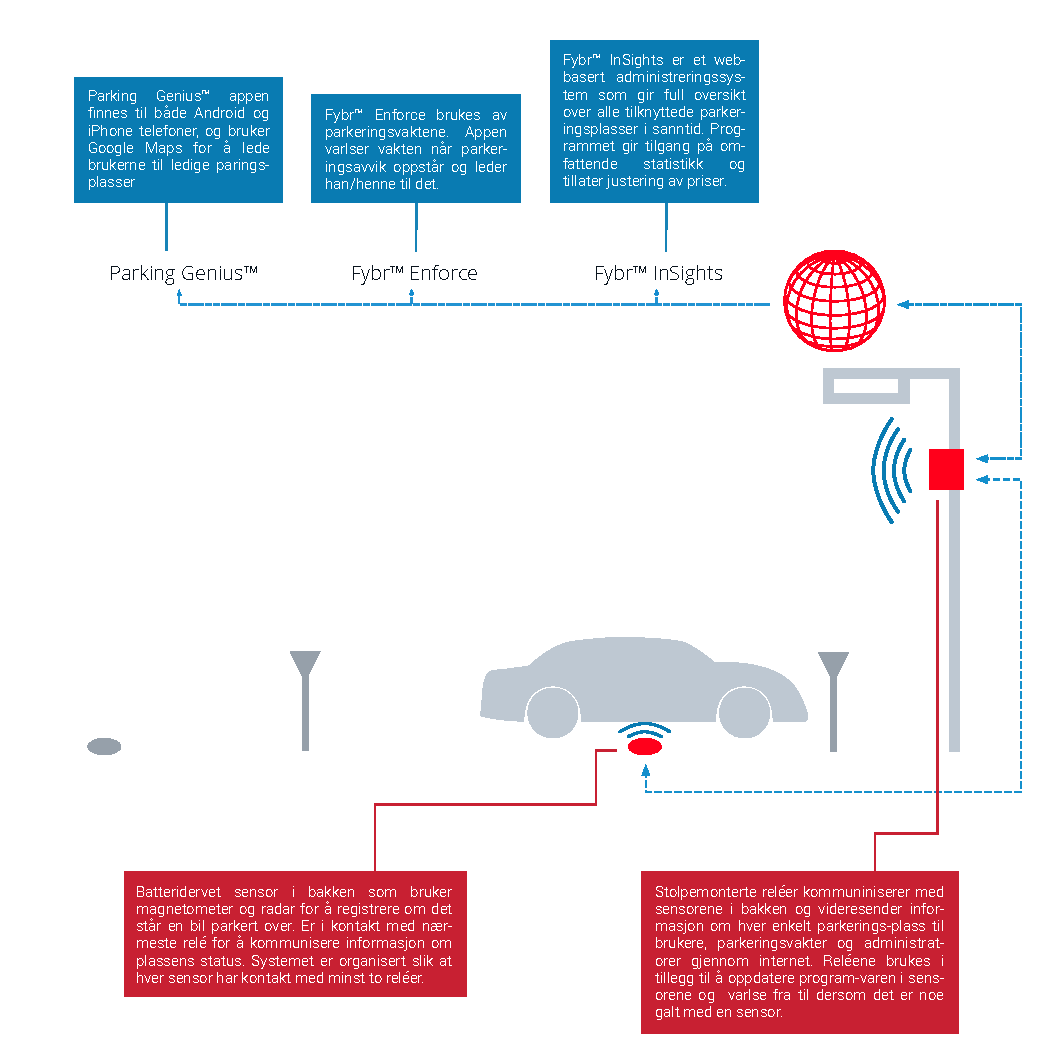
\includegraphics[scale=1.0, clip=true, trim=1cm 0.5cm 0.5cm 0.5cm]{grafikk/fybr.pdf}}
\end{figure}

Systemet måler overganger, altså når en bil ankommer eller forlater en parkeringsplass. Det kan registrere om parkeringsautomaten mottar betaling, men det ser ut til at dette baserer seg på det amerikanske systemet med en parkeringsautomat pr. parkeringsplass. I tillegg har systemet selvsagt oversikt over hvor lenge en bil har stått på en parkeringsplass; dette er svært nyttig for områder med tidsbegrenset parkering.

Sensorene benytter både magnetometer og rader for å registrere om en bil ankommer ellerforlater parkeringsplassen. De er batteridrevne, og kommuniserer med reléer montert høyt oppe på stolper. I tillegg til å kommunisere statusen for hver parkeringsplass til det sentrale systemet, brukes reléene til å oppdatere programvaren i sensorene. Batterilevetiden for sensorene er opp til fem år, og sensorene kan selv varsle dersom noe er galt. 

Datasystemet som følger med Fybrs parkeringssystem inkluderer tre verktøy som er nyttige for forskjellige interessenter:

\begin{itemize}
	\item Parking Genius, en mobilapp for iPhone og Android  som gir brukerne oppdatert informasjon om ledige parkeringsplasser, og viser veien til de.
	\item Fybr Insights er et webbasert administreringssystem som gir sanntidsinformasjon fra hele systemet, og lar etaten justere priser i sanntid dersom dette er ønskelig.
	\item Fybr Enforce er en mobilapp for parkeringsvakter som varsler når avvik oppstår og leder de til det.
\end{itemize}

Justeringen av priser i sanntid er ment å bidra til å sørge for at det alltid er en ledig plass i et område. Dette gjøres ved at prisene justeres opp i områder med mange oppdatte plasser, og ned i områder med mange ledige plasser, noe som oppfordrer folk til å parkere i i områder med mindre press.
% subsubsection fybr (end)


\clearpage
\subsubsection{SmartPark}
\label{ssub:smartpark}
SmartPark er en global leverandør av parkeringsløsninger, og har ett av sine kontor i Storbritannia. De har listet opp sine tidligere oppdrag på nettsiden, og noen av de vil kunne være interessante å se på siden de omhandler byparkering. I tillegg viser det at dette er en seriøs aktør innenfor parkeringsystemer. 

SmartPark sine sensorer som går under navnet SmartEye bruker infrarød teknologi(fungerer denne teknologien gjennom snødekke? samme med rfid leseren) for å oppdage om plassen er okkupert. Informasjonen som blir samlet inn av sensoren, blir så videresendt trådløst til en sone kontrollør for å minimere kostnader ved installasjon av SmartEye. Kontrollørene til hver sone videreformidler dataene til den sentrale serveren gjennom 3G. Sensoren bruker batteri som strømkilde, og batteriet har en levetid på rundt 5 år. 

\begin{figure}[H]
\centering
\centerline{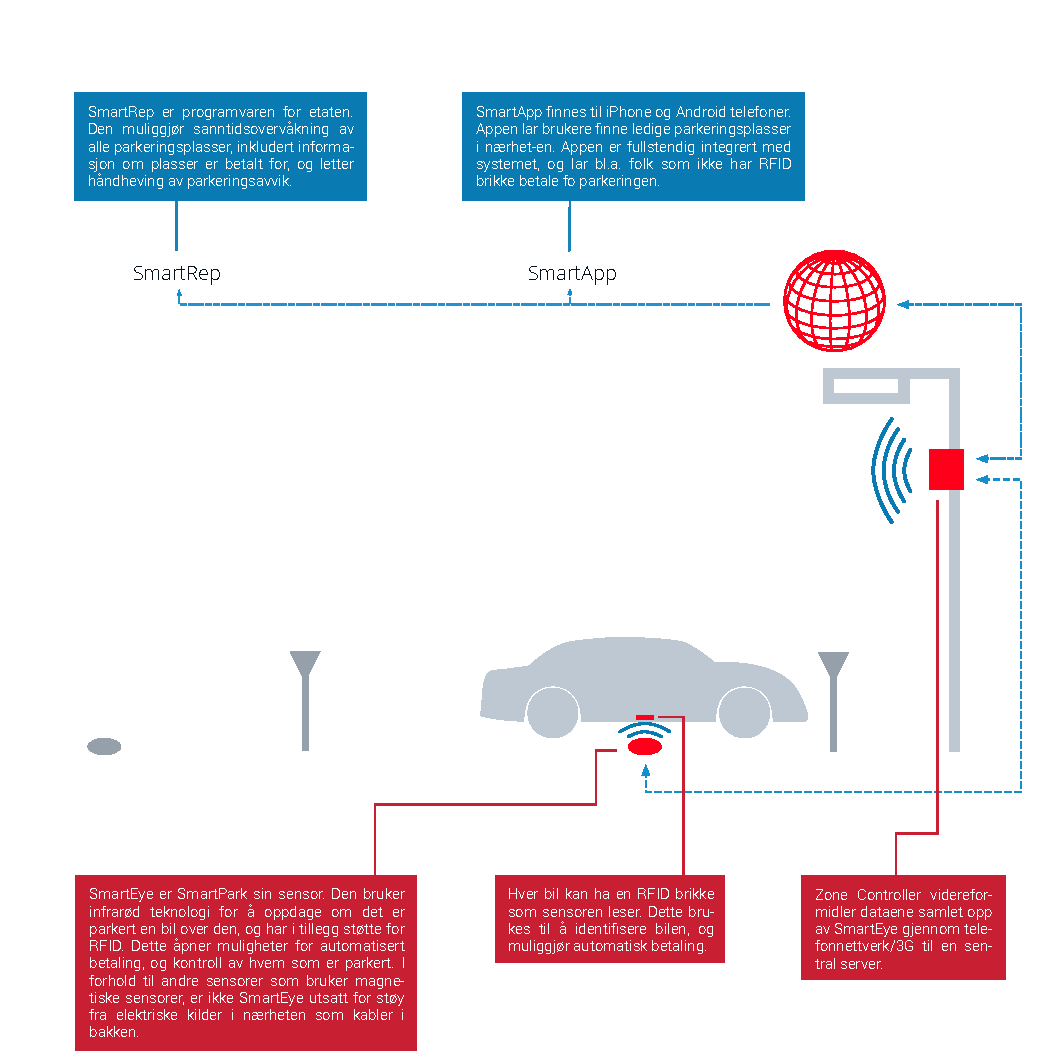
\includegraphics[scale=1.0, clip=true, trim=1cm 0cm 0.5cm 1.5cm]{grafikk/smartpark.pdf}}
\end{figure}

SmartPark pleier å levere pakkeløsninger med sensor og programvare. Programvaren rangerer ifra et program på datamaskinen til applikasjoner på telefon. Programvaren gir overblikk over hvilke plasser som er okkupert, og videreutvikles hele tiden for å kunne kjøre analyse på parkeringsmønstre. (Jobbtid mot “fritid”)
De har egne betalingsløsninger uten RFID vha egenutviklede parkometere. Man er ikke nødt til å kjøpe parkometrene for at sensorene skal kunne fungere(Sjekk?). I tillegg har de støtte for å bygge inn RFID i sensorene. Deres RFID system kobler en SmartEye sensor opp mot en bilist sin RFID tag. Dette kan brukes til å kunne automatisere betaling. 

% subsubsection smartpark (end)




\subsubsection{Urbiotica}
\label{ssub:urbiotica}
Urbiotica er en leverandør av sensorer for mer enn bare parkering. De går under “sloganet” The City Operating System, og har hatt et stort prosjekt på parkeing i Nice, Frankrike. Her er det over 10 000 plasser som er overvåket. Et annet nevnt prosjekt er til et kjøpesenter i Vienna som trengte kontroll av deres utendørs parkeringsområde. 

\begin{figure}[H]
\centering
\centerline{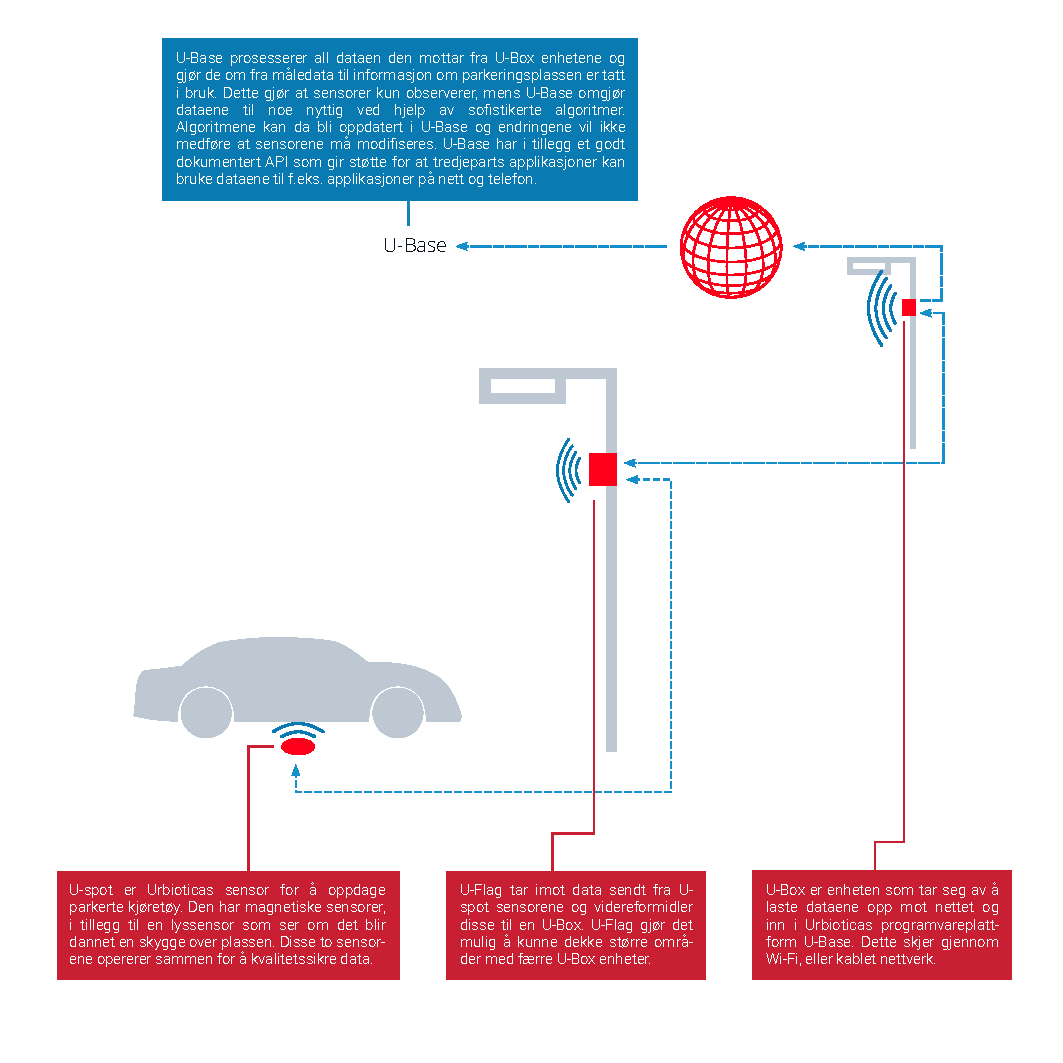
\includegraphics[scale=1.0, clip=true, trim=1cm 1.0cm 0.5cm 0.5cm]{grafikk/urbiotica.pdf}}
\end{figure}

Urbiotica sin tilnærming til parkeringsproblematikken inneholder fire sentrale komponenter. 
\begin{itemize}
	\item U-Spot, sensoren bruker magnetiske sensorer for å oppdage om det står en bil parkert ved eller over den. I tillegg bruker den en lyssensor for å kvalitetssikre dataen ved å forsikre seg om at det er en bil parkert og ikke et tilfeldig objekt av metall. Sensoren skal tåle ned mot -20 C, og kan plasseres opp til 50 meter ifra en U-Flag eller U-Box. Estimert levetid fra batteriprodusenten lå på rundt 10 år, og selve installasjonen av U-Spot kan gjøres i underkant av 10 minutter.   
	\item U-Flag, er en liten boks som kan festes på lyktestolper eller husvegger. U-Flag samler opp data fra sensorene og videresender denne dataen til en U-Box. Fungerer som en relè fra sensorene til U-Box’er. U-Flag kan være plassert opp til 100 meter ifra U-Box. Har strøm fra en fast kilde, f eks lyktestolpen, i tillegg til et batteri ved feil i strømnettet. 
 \item U-Box, enheten som har ansvaret for å sende de oppsamlede dataene gjennom WiFi til Urbioticas programvare-plattform som tar seg av lagringen. U-Box er også anbefalt å henges opp på lyktestolper eller husvegger slik som U-Flag, og bruker også strøm fra en fast kilde med et batteri i tilfelle strømnettet skulle oppleve feil. 
	\item U-Base, er enheten som prosesserer all dataen den mottar fra U-Box enhetene og transformerer de fra måledata til informasjon som forteller oss om parkeringsplassen er tatt i bruk. Dette deler opp ansvaret mellom enhetene slik at sensorene kun observerer, og U-Base omgjør dataene til noe nyttig ved hjelp av sofistikerte algoritmer. Algoritmene kan da endres på i U-Base uten at en er nødt til å kjøre en oppdatering av hver sensor hvis en skulle ha behov for det. U-base har i tillegg et godt dokumentert API som gir støtte for at tredjeparts applikasjoner kan bruke dataene til f.eks. applikasjoner på nett og telefon. 
\end{itemize}

De har også et siste element som heter U-Admin. U-Admin er Urbioticas programvare som skal guide brukeren gjennom installasjon av utstyret, og gi de mulighet til å få en visuell fremstilling av dataene som er samlet inn fra sensorene. Det gir også et overblikk over status på nettverket av sensorer, slik at man til en hver tid kan se hvordan det oppfører seg og om det er nødvendig å sende ut teknikere til sensorer. 

Siden Urbiotica driver med mer enn bare parkering, har man gode muligheter til utvidelse av systemet på andre områder enn bare trafikk. U-Flag/U-Box kan brukes sammen med andre sensorer som kan kontrollere nivå på avfall i søppelkontainere, luftfuktighet og generell trafikkflyt i byen. 

Det står ikke nevnt noe om støtte for RFID i U-Spot sensoren. (Sjekke i mail?) Det virker heller ikke som om dette er koblet opp mot et betalingssytem, så hvis en skulle brukt dette systemet må en definere hvordan betaling skal fungere. 



% subsubsection urbiotica (end)







% subsection sksisterende_systemer (end)



% section teknologi (end)





\section{Forslag til implementering}
\label{sec:implementering}

% section implementering (end)





\section{Diskusjon}
\label{sec:diskusjon}

% section diskusjon (end)






\section{Konklusjon}
\label{sec:konklusjon}

% section konklusjon (end)






\pagebreak
\bibliography{referanser.bib}{}
\bibliographystyle{unsrt}
\pagebreak




\appendix

\section{Første appendix}
\label{sec:}

% section  (end)


\end{document}






































